% id: 48-05
% book: 100발100중 3-2 기말 · 01 3-2 기말(원의 성질·통계·부록)
% section: 기출 Best 쌍둥이
% figure: crop:fig-48-05.png
% answer: ③
% answer_source: 답지(빠른정답)
% variant_level: 0 (원본 전사)
% 이 파일은 build.mjs 가 items.json 에서 만든다. 고칠 때는 items.json 을 고친다.
\smash{\raisebox{1.5mm}{\dmkichul{100발100중 3-2 기말 48쪽 05번 · 동영상}}}
\noindent\begin{minipage}[t]{0.58\linewidth}\vspace{0pt}\raggedright 그림은 학생 $20$명의 영어 수행평가 점수를 조사하여 막대그래프로 나타낸 것이다. 중앙값을 $m$점, 최빈값을 $n$점이라 할 때, $m+n$의 값은?\end{minipage}\hfill\begin{minipage}[t]{0.4\linewidth}\vspace{0pt}\centering 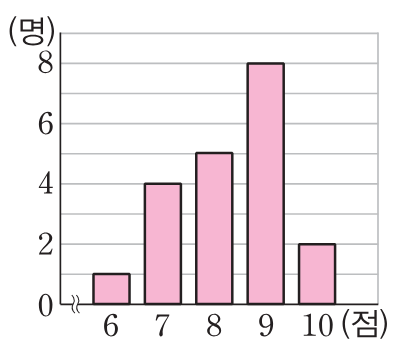
\includegraphics[width=95.2pt]{figures/fig-48-05.png}\end{minipage}\par
\begin{choices32}{$16$}{$17$}{$17.5$}{$18$}{$18.5$}\end{choices32}
